\documentclass{uhphyspaper} 
%%%%%%%%%%%%%%%%%%%%%%%%%%%%%%
%       START DOCUMENT       %
%%%%%%%%%%%%%%%%%%%%%%%%%%%%%%
\usepackage{lipsum} % For demo purposes, remove 
\usepackage{listings} % Provides \lstinline{} for demo, remove

% Titles
\title{Title (bold)*}
\runningtitle{*Running title: \textit{Short title ($\mathit{< 50}$ characters inc. spaces, italic, leave empty if not needed)}}
\keywords{list at least five keywords, separated by commas}

% Course information
\bachyear{$\mathit{3^{e}}$}
\course{Bachelorproef}
\date{\today}

% Authors, supervisors, principle investigator (PI, promotor)
\author[1]{Student Name}
\author[2]{Supervisor name}
\author[3]{Second supervisor}
\author[4$^{\dagger}$]{Principle Investigator} % Promotor: Dagger here signifies that the PI is the main correspondent

% Author affiliations
\affil[1]{UHasselt, Agoralaan, 3590 Diepenbeek, Belgium}
\affil[2, 3]{Specify Group}
\affil[1,4$^{\dagger}$]{UHasselt, ResearchGroup, Agoralaan, 3590 Diepenbeek, Belgium} % Dagger here signifies that the PI is the main correspondent

% PI contact info, do not remove
\pimail{PImail@uhasselt.be}


%%%%%%%%%%%%%%%%%%%%%%%%%%%%%%
%       START DOCUMENT       %
%%%%%%%%%%%%%%%%%%%%%%%%%%%%%%
\begin{document}
\maketitle\thispagestyle{fancy} % pagestyle ensures header is present

% Each section is placed in a separate file to better organise your text
% You can find these files in the Sections folder
\section{INTRODUCTION}
% Edit below
Leid je project in, background, doel \& onderzoeksvragen, \dots 
Zorg voor voldoende referenties zoals \cite{knuth:1984} \cite{latex2e}(Endnote/Mendeley/Zotero).
\section{THEORY (optional)}
% Edit below
Tussentitels zijn aangeraden per onderdeel (2.1, 2.2, \dots).
Zijn er essentiele stukken theorie die noodzakelijk zijn om je verslag te begrijpen?

Vergelijkingen doe je typisch met de align environment.
Dit laat je toe om \& (en \&\&) te gebruiken om alles mooi uit te lijnen.
    \begin{align}
    x \times x   &= (x \times x) + 0  &&\textit{ Neutr. El. }+\\
            &= (x \times x) + (x \times \neg x) && \textit{ Compl. }\times \\
            &= x + (x \times \neg x) && \textit{ Distr. }+ \\
            &= x + 0 && \textit{ Compl. }\times\\
            &= x && \textit{ Neutr. El. }+
    \end{align}
Wil je midden in een regel een vergelijking gebruiken doe het dan als volgt: $S = k\ln(W)$ % May be removed if unnecessary
\section{EXPERIMENTAL PROCEDURES}
% Edit below
Tussentitels per techniek (3.1, 3.2, \dots).
Welke technieken zijn er gebruikt?
Zorg dat je onderzoek repliceerbaar is (maar zonder overbodige details).
\begin{figure}[H]
    \centering
    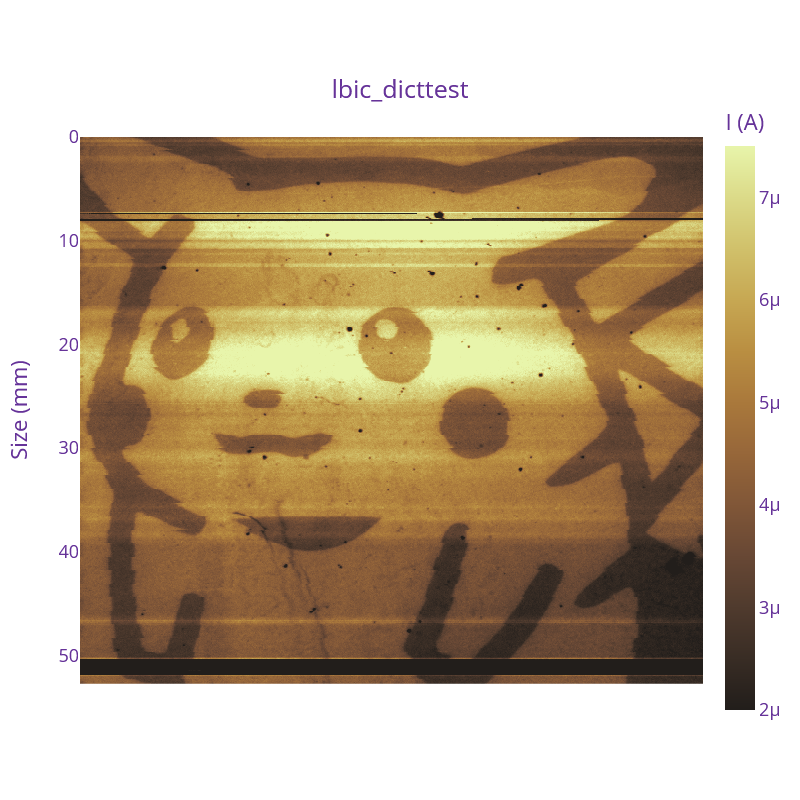
\includegraphics[width=\linewidth]{Figures/newplot(4).png}
    \caption{Caption}
    \label{fig:my_label}
\end{figure} % May be removed if unnecessary
\section{RESULTS}
% Edit below
Tussentitels per topic/techniek (4.1, 4.1.1, \dots).
Beschrijf de resultaten (interpreteer ze nog niet), wat zie je (objectief)?
Zorg dat figuren een caption hebben (incl. alle afkortingen) onder de figuur en dat je zeker in de tekst refereert naar desbetreffende figuur. 
Tabellen krijgen een caption bovenaan (zelfde principe).

Willen jullie resultaten tonen zoals figuren dan dienen jullie de \textit{figure} environment gebruiken.
\begin{figure}
    \centering
    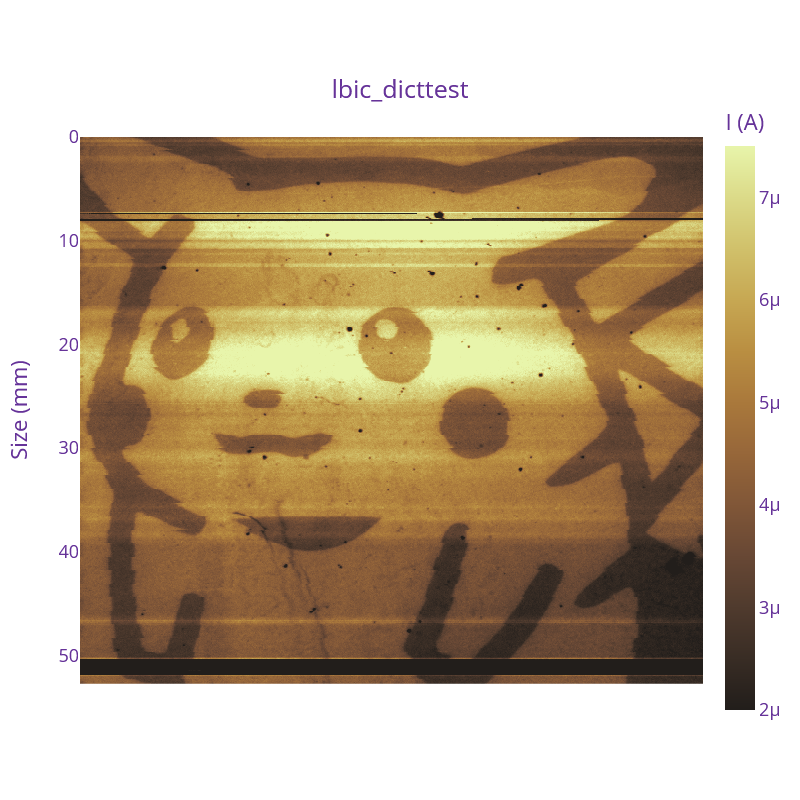
\includegraphics[width=\linewidth]{Figures/newplot(4).png}
    \caption{Dit is het onderschrift van deze figuur}
    \label{fig:pikachu}
\end{figure}

Je kan naar een figuur refereren met \lstinline!\cref{fig:pikachu}! door een label te plaatsen in je figure environment: \lstinline!\label{fig:pikachu}!.
\Cref{fig:p1,fig:p2} toont hoe eventueel gebruik gemaakt kan worden van \textit{minipage} voor twee zij-aan-zij figuren.
\begin{figure*}[!htpb]
    \centering
    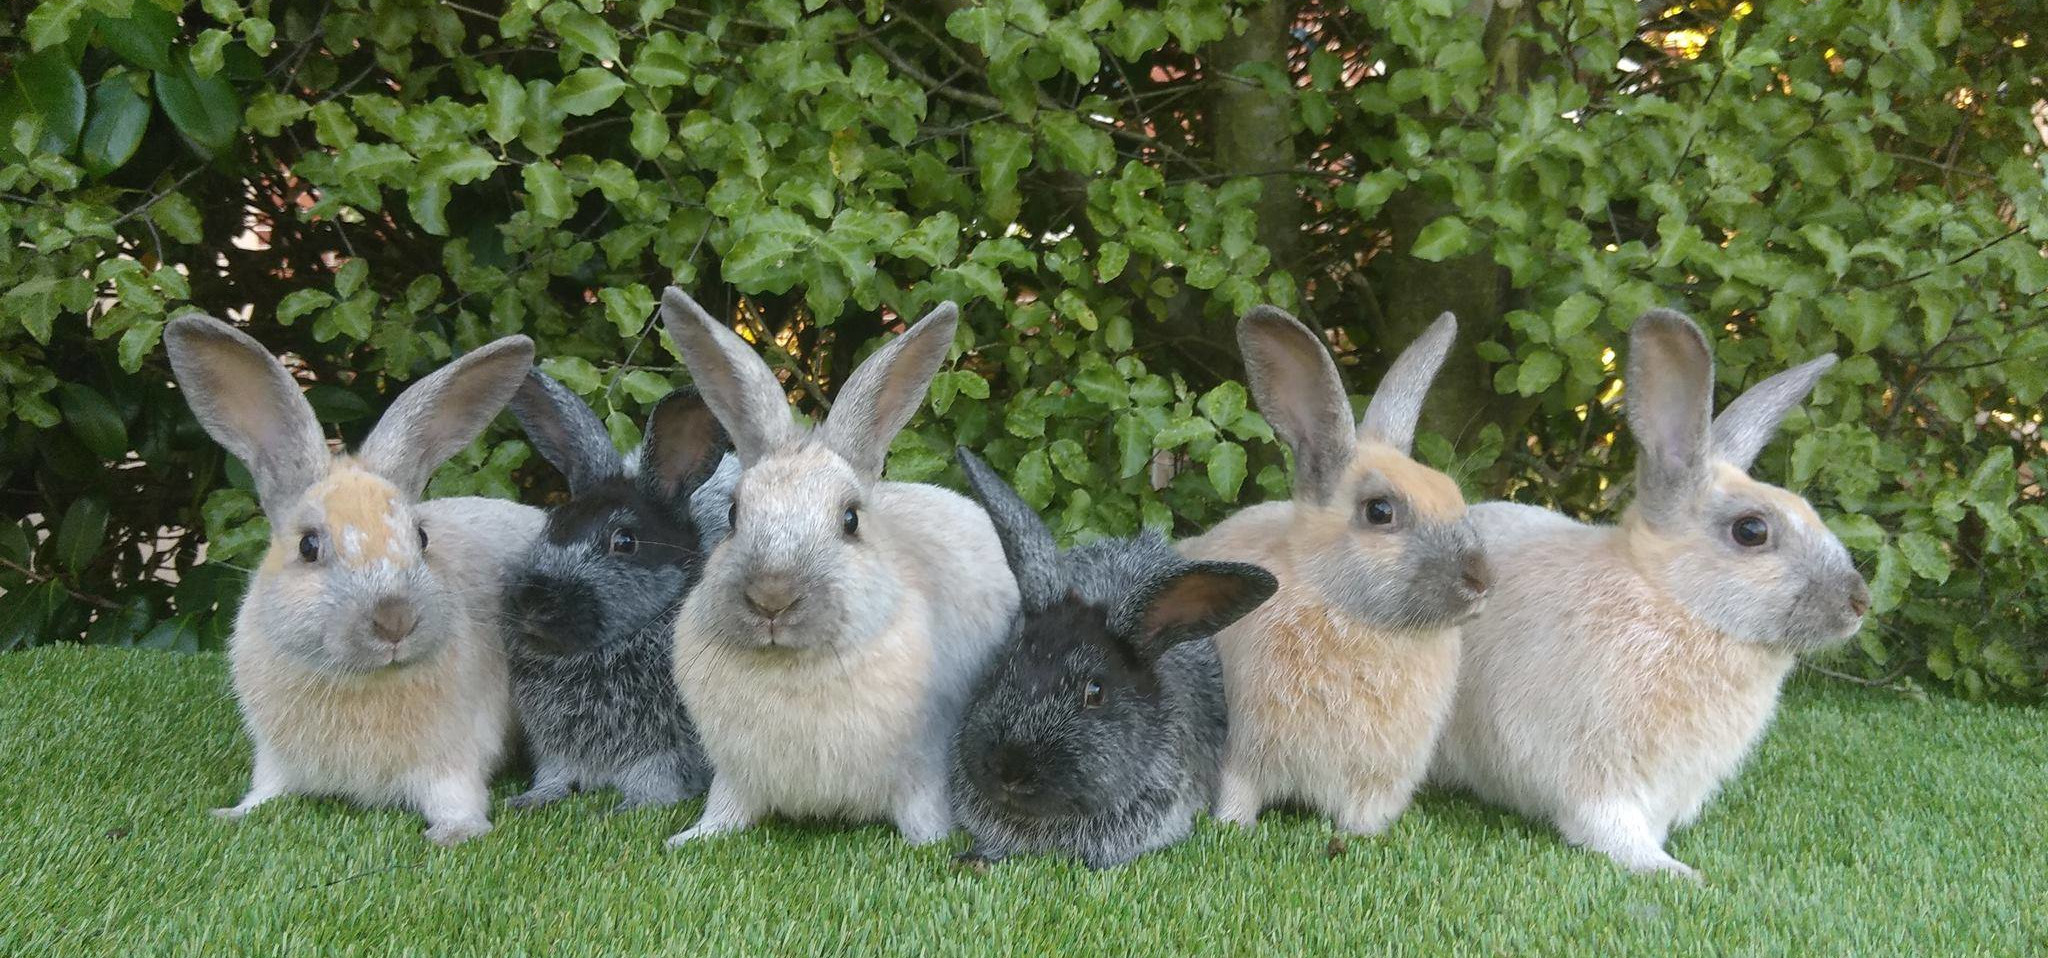
\includegraphics[width=\textwidth]{Figures/Enderby_Island_Rabbit_Lineup.jpg}
    \caption{Dit is een veel te grote figuur. Konijnen zijn belangrijk en moeten de hele pagina innemen.}
    \label{fig:konijnen}
\end{figure*}

\begin{figure*}
    \centering
    \begin{minipage}{0.45\textwidth}
        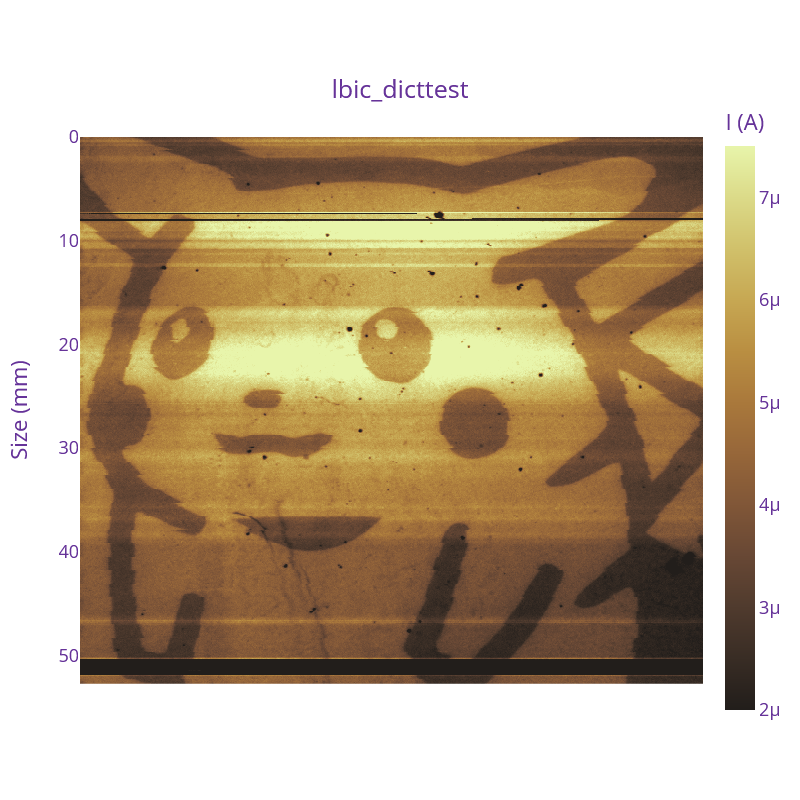
\includegraphics[width=\linewidth]{Figures/newplot(4).png}
        \caption{Dit is het onderschrift van deze figuur}
        \label{fig:p1}
    \end{minipage}
    \hspace{0.05\textwidth}
    \begin{minipage}{0.45\textwidth}
        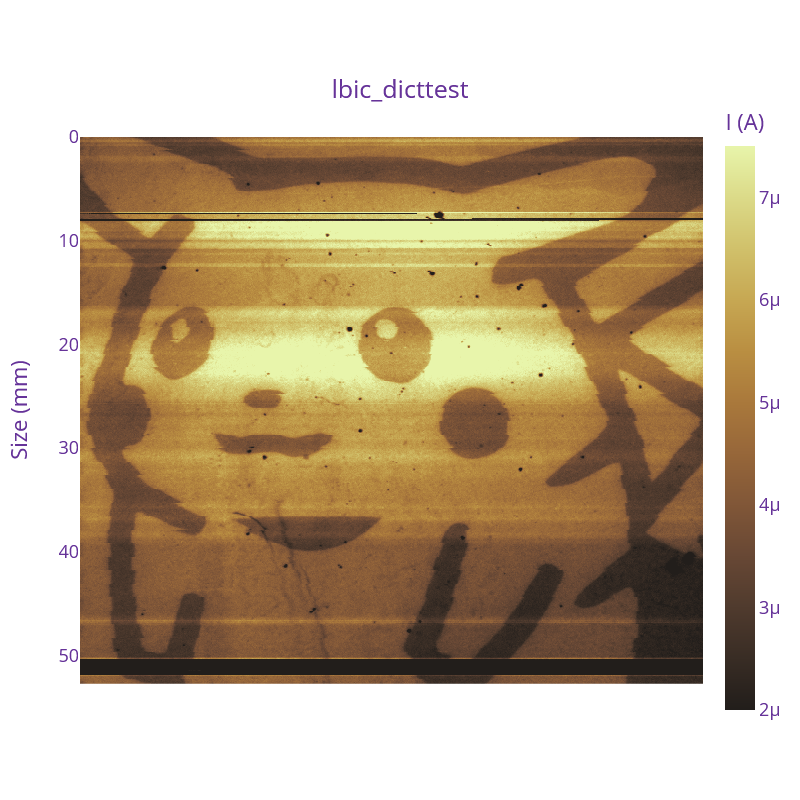
\includegraphics[width=\linewidth]{Figures/newplot(4).png}
        \caption{Dit is het onderschrift van deze figuur}
        \label{fig:p2}
    \end{minipage}
\end{figure*}

Tabellen moeten in de \textit{table} environment geplaatst worden.
Ook hier is de 'H' parameter cruciaal.
Gebruik \url{https://www.tablesgenerator.com/} voor hulp bij de opmaak van tabellen.
\begin{table}[H]
\centering
    \label{tab:example_table}
    \caption{Example table with no meaning}
    \begin{tabular}{||c c c c||} 
    \hline
    Col1 & Col2 & Col2 & Col3 \\ [0.5ex] 
    \hline\hline
    1 & 6 & 87837 & 787 \\ 
    2 & 7 & 78 & 5415 \\
    3 & 545 & 778 & 7507 \\
    4 & 545 & 18744 & 7560 \\
    5 & 88 & 788 & 6344 \\ [1ex] 
    \hline
    \end{tabular}
\end{table}
\section{DISCUSSION}
% Edit below
Tussentitels aangeraden.
Beschrijf welke conclusies er getrokken kunnen worden uit je resultaten. 
Leg linken (zowel tussen je eigen resultaten als dingen die je vindt in de literatuur).
\npar
Ook hier is extra voorbeeldtext: \lipsum[1-1]
\section{CONCLUSION}
% Edit below
Kort en bondig, wat leren we hier uit? 
Wat is de outlook?

% Additional sections for acknowledgments
\rule{\linewidth}{0.4pt}
\textit{Author contributions} -- \textbf{Who did what?} 
% Edit below
JH and JdR conceived and designed the research. 
JH and BvH performed experiments and data analysis. 
EvS and DD provided assistance with FLIM-FRET. JH and JdR wrote the paper. 
All authors carefully edited the manuscript.

\textit{Acknowledgements} -- \textbf{Who helped you? Who do you want to thank.} 
% Edit below
F.E. BvH acknowledges the agency for Innovation by Science and Technology (IWT Flanders) for his doctoral fellowship. 
JH is grateful for a postdoctoral scholarship from the Research Foundation Flanders (FWO Vlaanderen). 
Prof. Em. Yves Engelborghs is thanked for providing access to the confocal microscope. 
Research was funded by grants from the BOF UHasselt, etc.

% The bibliography is added at the end of the paper in a single column
\vspace{0.5cm}
\printbibliography[title={REFERENCES}]

\end{document}